\clearpage
\section{High frequency measurement on Tantalum Resonator}

In this section, the Tantalum resonator is made and measured. We fabricate 12 Tantalum resonators with a common feedline on the sapphire substrate. Then we load it into the dilution refrigerator, extract the forward transmission signal and fit the data with the resonator model. The measurement is all done in QDev's Triton 2 dilution fridge.

\subsection{Calibration on readout input line's attenuation before loading}

The high-frequency measurement is sensitive to the wiring in the fridge and shielding. To accurately calculate the photon number loaded into the resonator, we have to know the exact attenuation on the readout input line. The calibration is done by shorting the drive line and an unattenuated line, then measuring the transmission rate S21 on VNA. The drive line has in total of 60 dB attenuators and approximately 20 dB attenuation on others when calibrating at 7GHz at the base temperature in the dilution fridge.
\begin{figure}[h!]
    \centering
    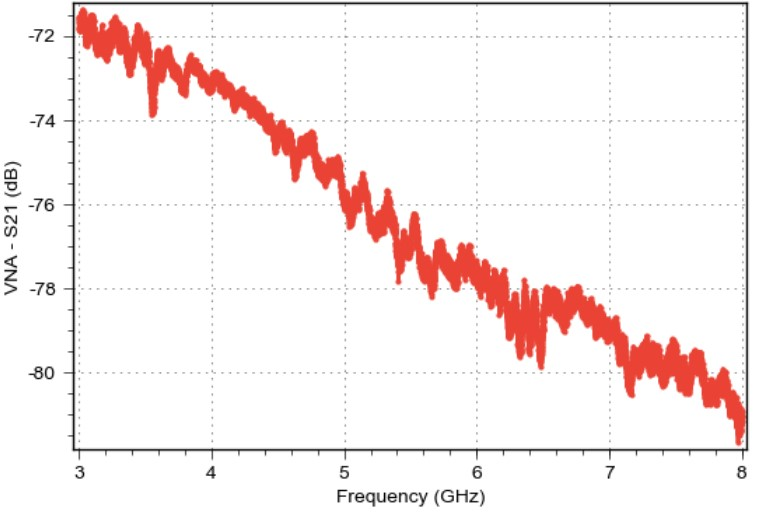
\includegraphics[width=0.6\textwidth]{Pic/Cali_res.jpg}
    \caption{The transmission on the T2 fridge was measured on VNA. The resonators are lying between 6-7 GHz, so the total attenuation on line is around 80 dB.}
    \label{fig:my_label}
\end{figure}

\subsection{Fitting function for extracting Q factor}
\begin{figure}[h!]
    \centering
    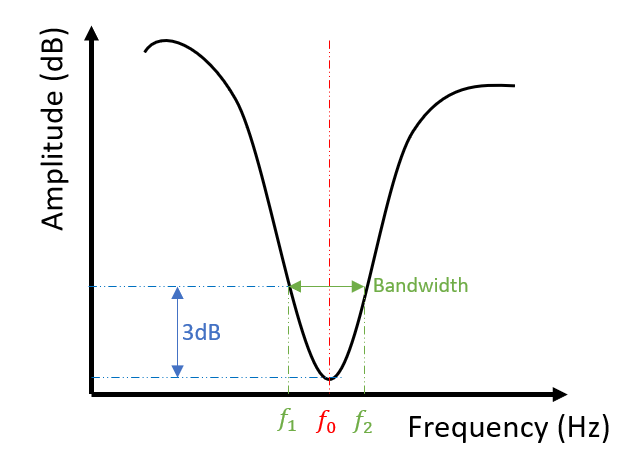
\includegraphics[width=0.6\textwidth]{Pic/3dB_est.png}
    \caption{The diagram shows the components we need to estimate the loaded quality factor.}
    \label{estQL}
\end{figure}
Quantum fitter, the package we make for data fitting, is perfect for routine usage on fitting high-frequency measurement data and plotting them. The resonator fitting formula, considering non-ideal elements such as impedance mismatch, can be described as\cite{RN64, RN66}:
\begin{equation}\label{ResonatorFit}
    S_{21} = A \left(1 + \alpha \frac{f-f_r}{f_r}\right)\left(1-\frac{\frac{Q_L}{|Q_e|}e^{i\theta}}{1+2iQ_L\frac{f-f_r}{f_r}}\right) e^{i(\phi_\nu f + \phi_0)}
\end{equation}
Here the quality factor $Q_L$ is the important parameter with relation $1/Q_L = 1/Q_i + 1/Q_c$, where $1/Q_i$ is the internal quality factor that tells us the intrinsic decay rate of the resonator, and $Q_e$ indicates the coupling between resonator and the feedline with $Q_e = |Q_e|e^{i\theta}$ (asymmetry in the resonator line shape) and $1/Q_c = \text{Re}(1/Q_e)$. The higher $Q_i$ is in low readout power, the better resonator we get. To obtain a trustworthy internal quality factor, we need to modulate the external quality factor to the same order. Therefore we have 12 resonators with different coupling strengths to the feedline. 

The loaded quality factor is simply estimated by measuring the 3 dB cut-off frequency at the resonance peak (Fig.\ref{estQL}). The definition of loaded quality factor in power is $Q_L = f_r / \Delta f$, where $f_r$ is the resonance frequency, and $\Delta f$ is the full width at half maximum (FWHM) frequency. The definition of dB is:
\begin{equation}
    L = 10 \log_{10}\frac{P}{P_0} (dB)
\end{equation}
Consequently, 3 dB is equivalent to a half drop of power $P/P_0 = 0.5$, which is the FWHM we need. With the formula:
\begin{equation}
    Q_L = f_0 / (f_2 - f_1)
\end{equation}
we can calculate the rough quality factor of the system and use it to check if the fitting is valid.


\subsection{Measurement on bare resonators}
After fabrication of the Tantalum resonators 
on the chip, we immediately bond and load the resonator into T2. 
\begin{figure}[h!]
    \centering
    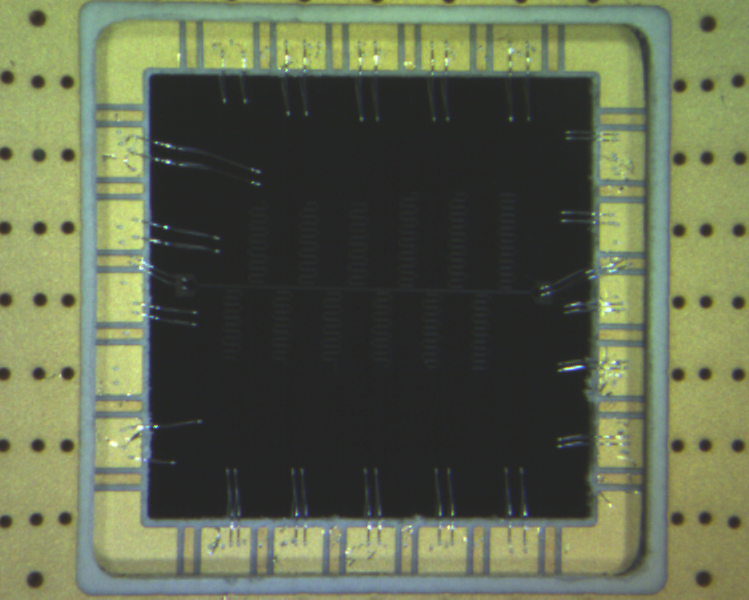
\includegraphics[width=0.6\textwidth]{Pic/Res_bond.png}
    \caption{The chip with bare resonators after bonding on the QCage board.}
    \label{fig:my_label}
\end{figure}
The first task is to find the 12 resonance dips on the overall resonator scan. The VNA is set to have no average with large bandwidth and scan over the 4 GHz range to find the resonance peak on the $S_{21}$ spectrum.
\begin{figure}[h!]
    \centering
    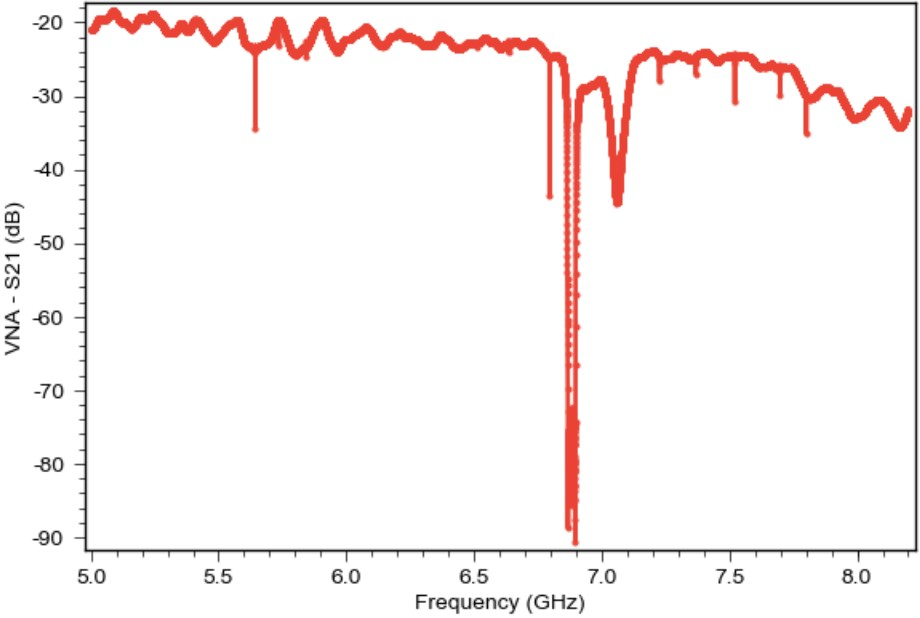
\includegraphics[width=0.6\textwidth]{Pic/Overall_res.jpg}
    \caption{Overall scan of the resonator. The resonance peak at around 6.9 GHz is the TWPA's eigenfrequency. Our design of the resonator has avoided the frequency around this peak.}
    \label{fig:my_label}
\end{figure}
After that, we do a finer scan on each resonator in high power to locate precisely the center frequency of all the resonators. Then we set a scan on the center frequency, with a small frequency span and low bandwidth, to measure the S21 on each resonator and fit it with the resonator model. 

\begin{figure}[h!]
    \centering
    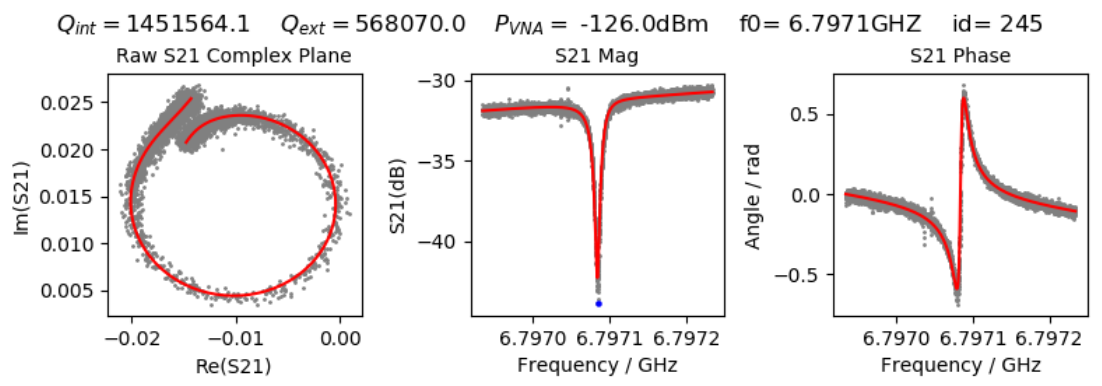
\includegraphics[width=0.9\textwidth]{Pic/Res_beforeclean_0.png}
    \caption{The fitting data with -46 dBm output from VNA. The total readout power to the resonators is -126 dBm.}
    \label{fig:my_label}
\end{figure}

\begin{figure}[h!]
    \centering
    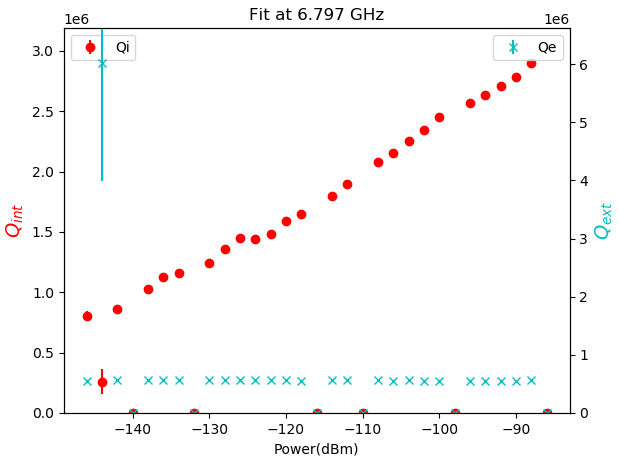
\includegraphics[width=0.7\textwidth]{Pic/Res_beforeclean.png}
    \caption{The fit down to -146 dBm. Now the VNA is attached with a 36dBm attenuator to reach a lower drive power.}
    \label{Fitallbare}
\end{figure}
The resonator has a decent internal Q while in high power but decreases dramatically while we approach the single photon regime. The figure shows the highest Q internal factor resonator on-chip, and the signal becomes too weak to measure below -146 dBm, roughly equal to 5 photons inside the resonator.

To get a higher Q internal factor, we unload the chip and do surgery on the chip and wiring.

\subsection{Measurement on post-cleaned resonators}

The high-frequency measurements, including resonator and qubit spectroscopy, are sensitive to environmental noise like Johnson–Nyquist noise, and TLS embedded in the material\cite{RN29}. Therefore, several strategies to reduce the noise on the chip are deployed. The chip is cleaned with Piranha solution for 20 minutes to reduce the quantity of reactivity metal like zinc and chemical compound residue from the fabrication process on the surface. \cite{RN67}. We then bonded the chip with on-chip bonds on both the feedline and the resonator. This technique helps to balance the voltage difference between two ground planes. Beyond these, we add the 50$\Omega$ terminator at the end of the SMP connector coaxial line to stop signal reflection to the chip and prevent noise from getting into the ground plane. 

\begin{figure}[h!]
    \centering
    \begin{subfigure}[b]{0.48\textwidth}
         \centering
         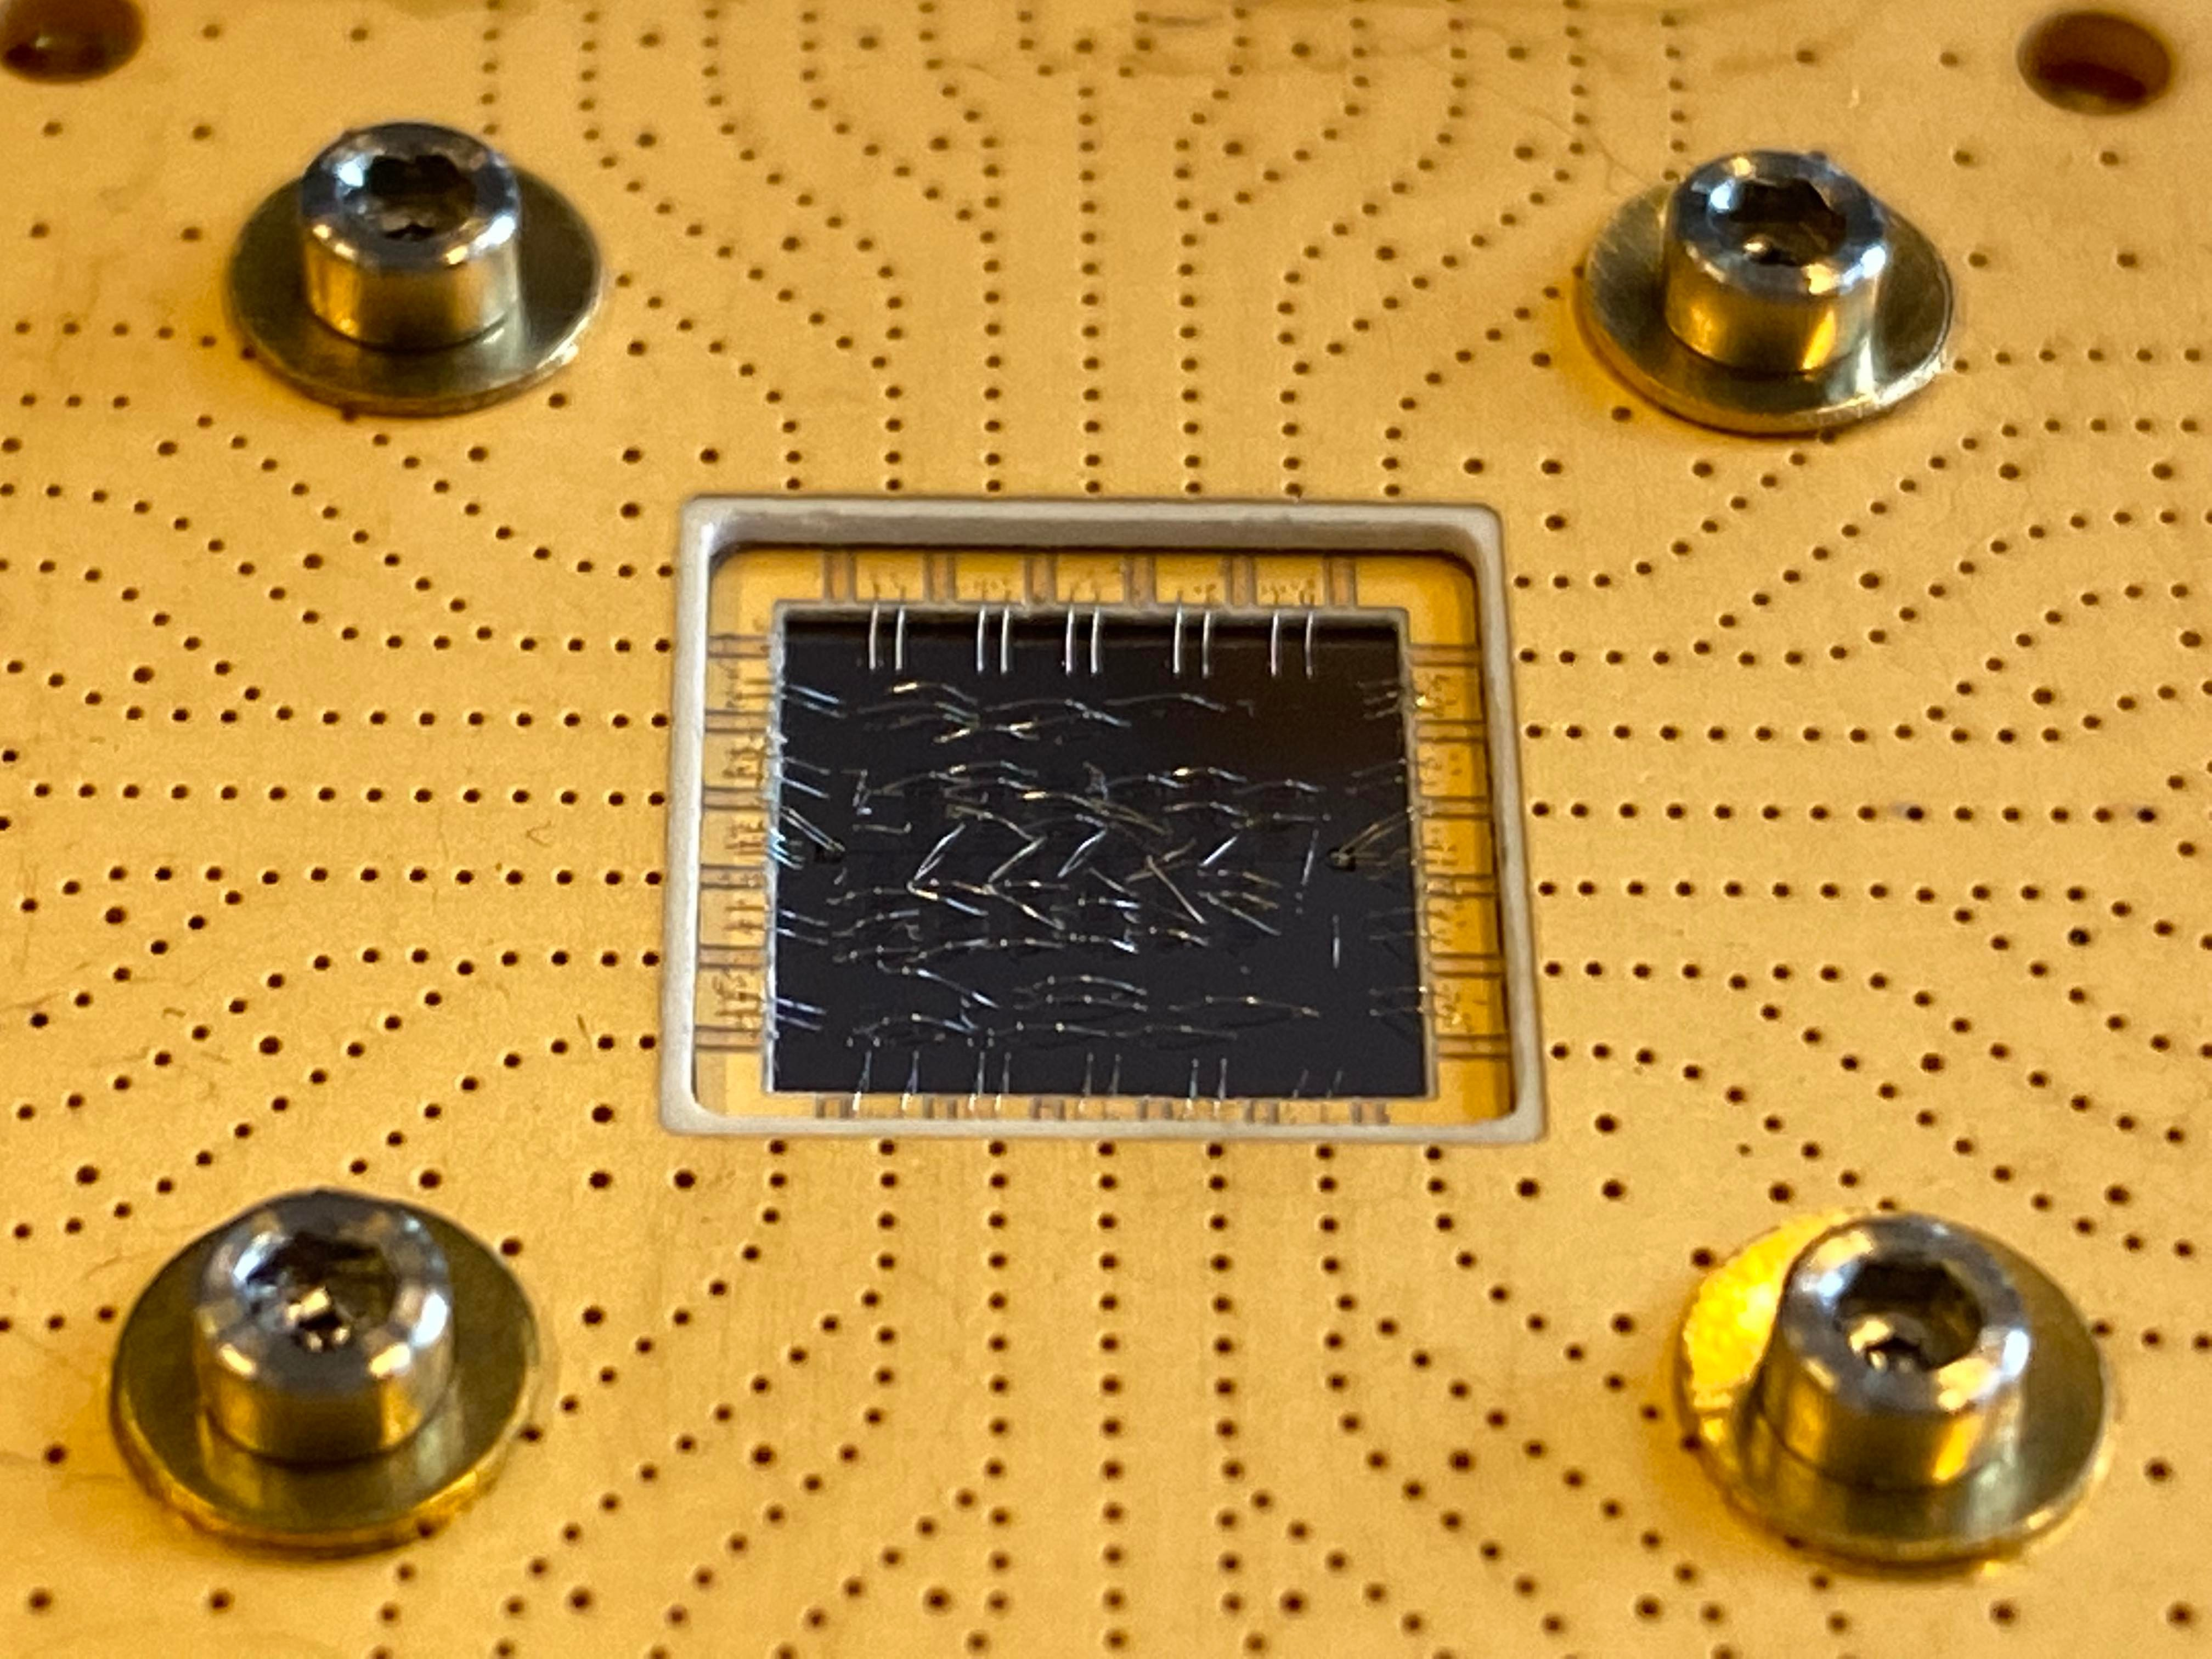
\includegraphics[width=\textwidth]{Pic/Res_postclean.jpg}
         \caption{}
         \label{OnchipBond}
     \end{subfigure}
     \hfill
     \begin{subfigure}[b]{0.48\textwidth}
         \centering
         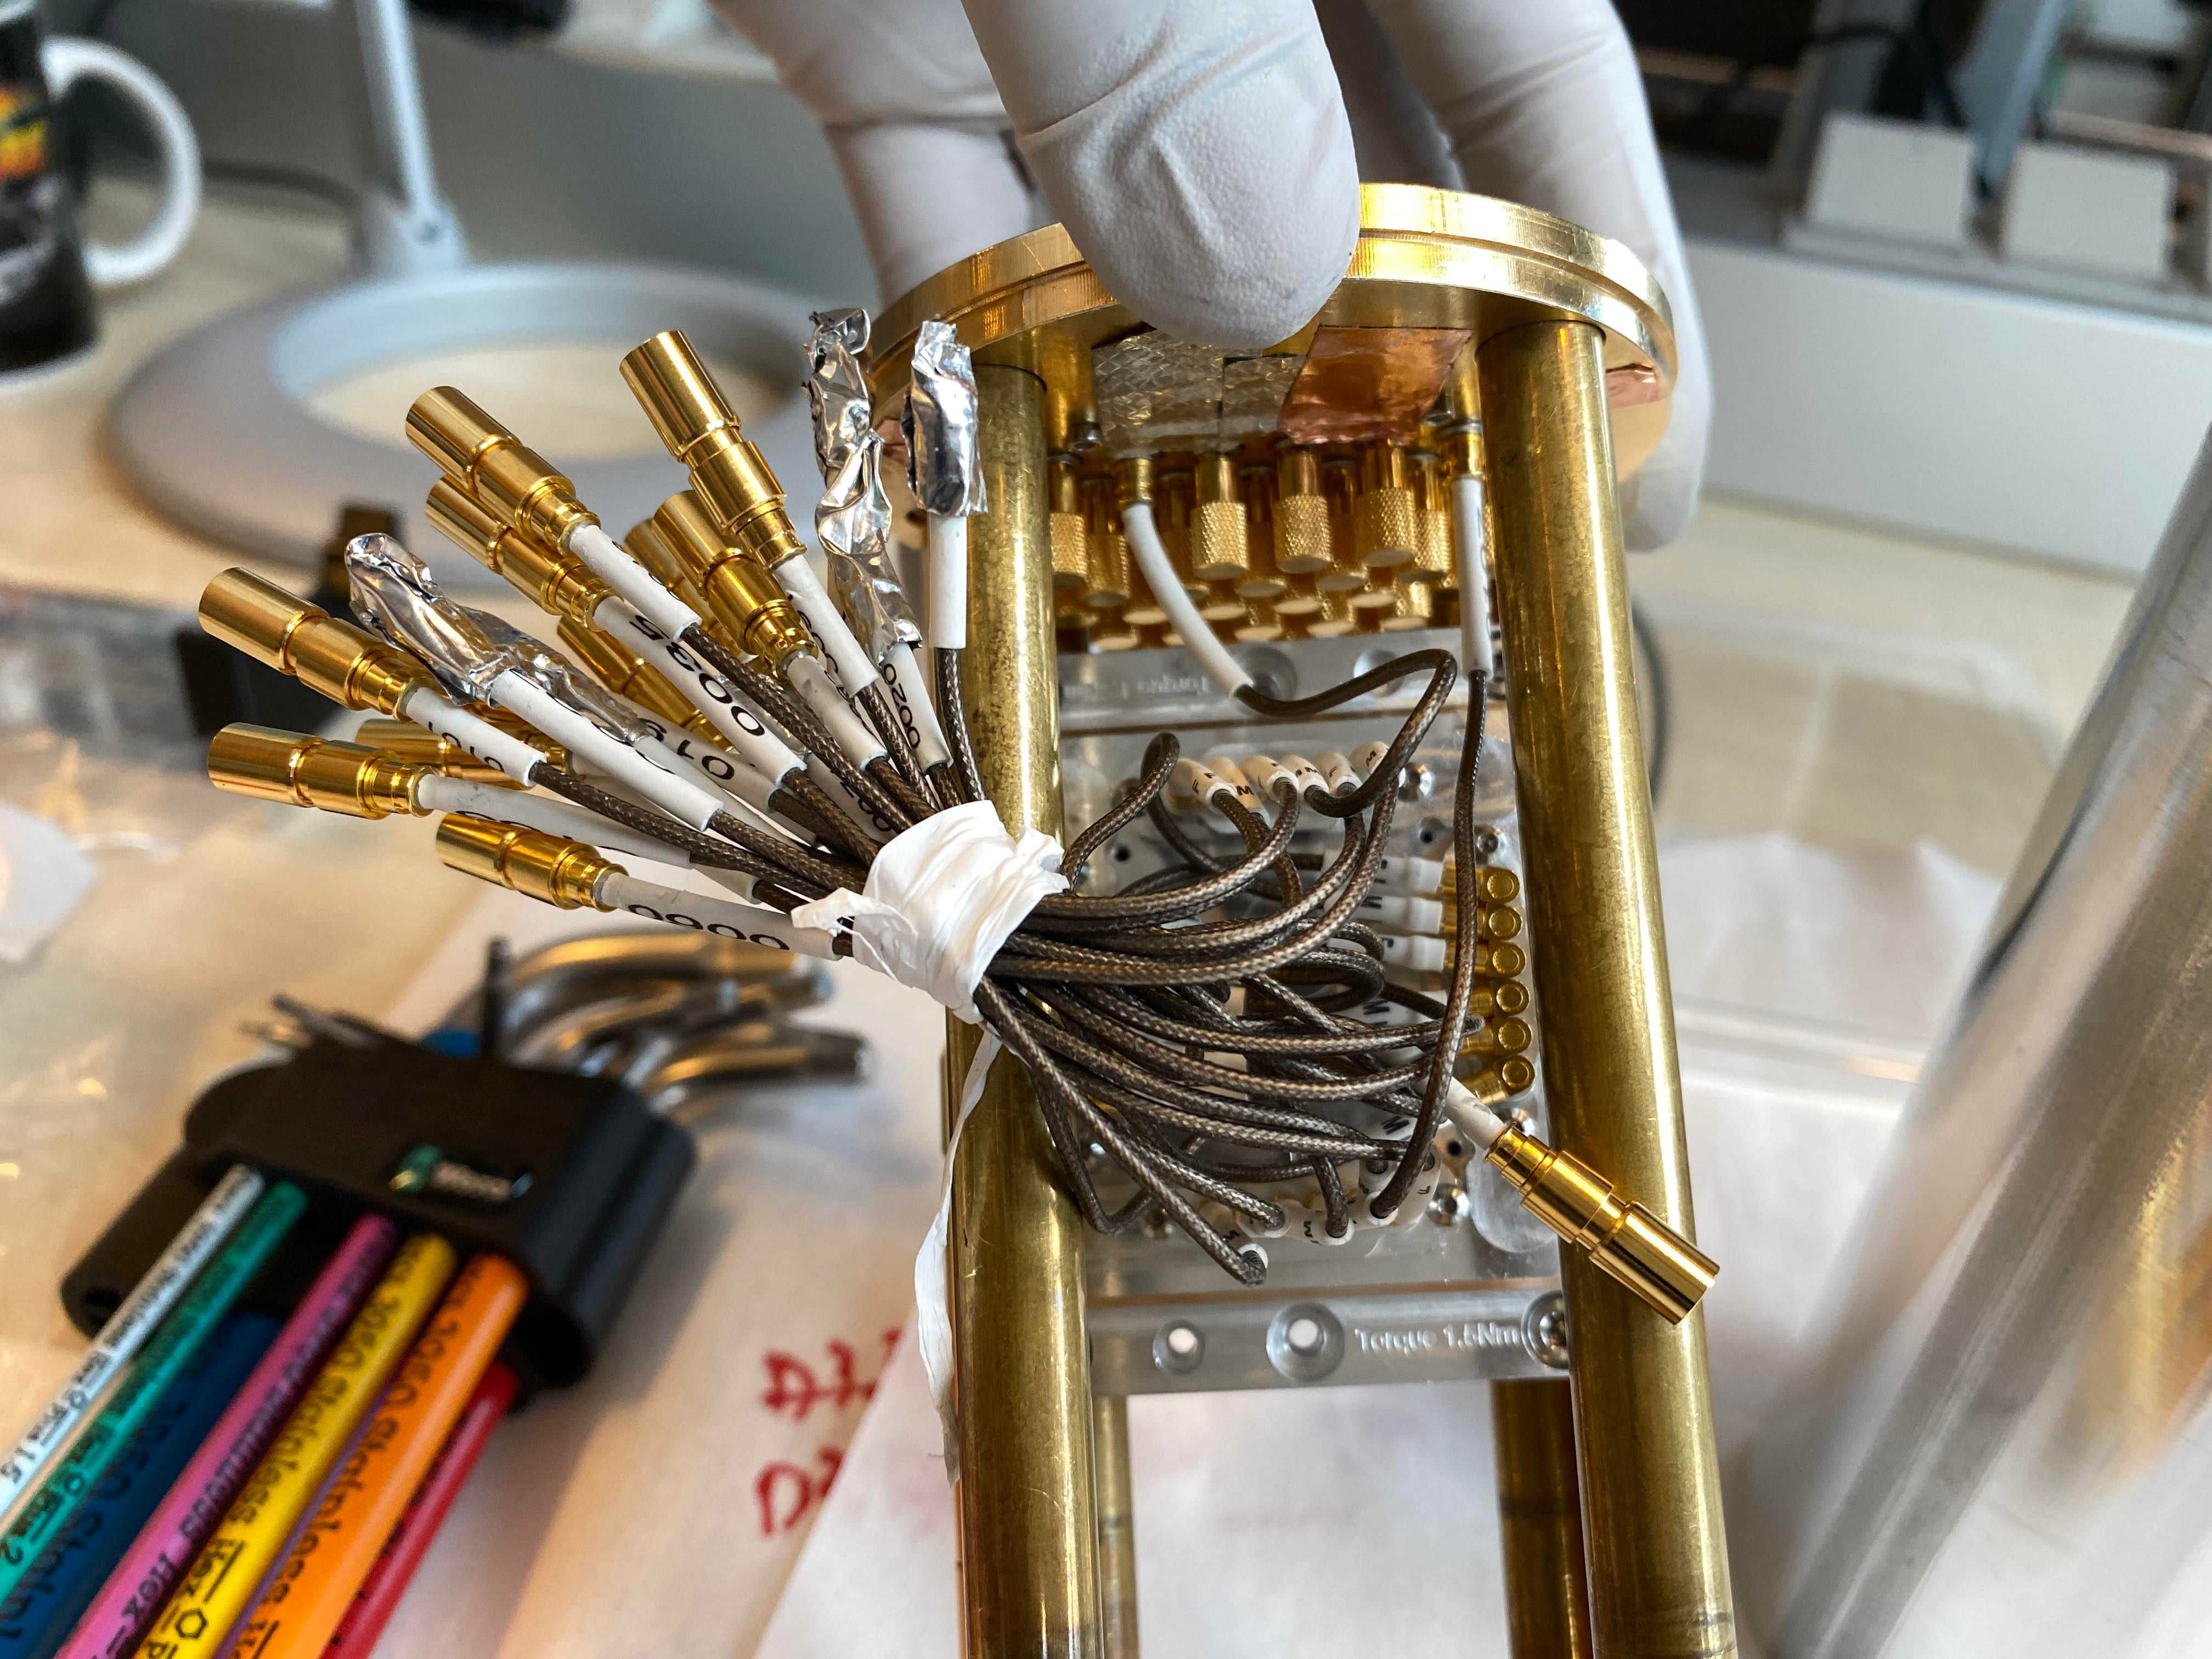
\includegraphics[width=\textwidth]{Pic/Res_termi.jpg}
         \caption{}
         \label{Terminator}
     \end{subfigure}
    \caption{(a) The on-chip bonding. Every resonator is cross-bonded with 2 to 3 bonding wires, and the feedline is cross-bonded with five bonding wires. (b) The $50\Omega$ terminators at the end of the SMP connector.}
    \label{TaNWonchip2}
\end{figure}

With this cleaning combination, the resonators gain a higher SNR and can measure down to a single photon regime. At -146 dBm, the $Q_i$ is nearly 1 million but around 800 thousand without the combination.

\begin{figure}[h!]
    \centering
    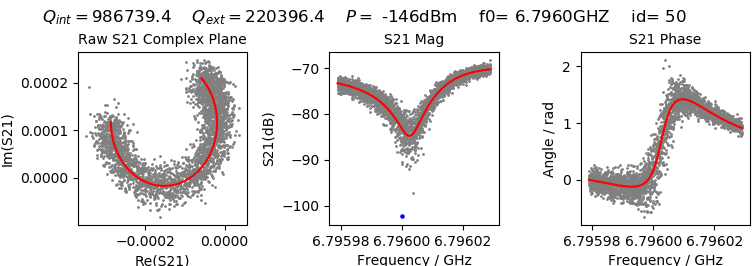
\includegraphics[width=\textwidth]{Pic/Res_postclean_0.png}
    \caption{The resonator fit in the post-clean resonator, which is better than the internal quality factor we showed on Fig \ref{Fitallbare}. At this power, the photon number inside the resonator is around 2.}
    \label{fig:my_label}
\end{figure}

Now the best resonator on the chip is around 7.8 GHz and still has over a million Q factors in the single photon regime (in this case, at -150 dBm).

\begin{figure}[h!]
    \centering
    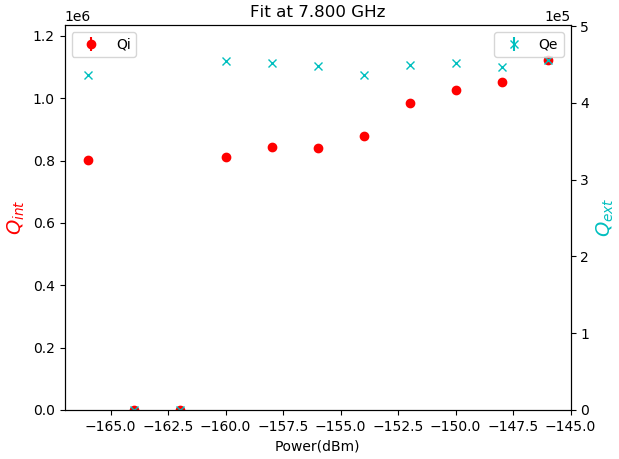
\includegraphics[width=0.8\textwidth]{Pic/Res_postclean_1.png}
    \caption{The fitting of the best resonator we find on chip. At -150 dBm, the resonator reaches the single photon regime and still has over a million internal quality factor.}
    \label{fig:my_label}
\end{figure}

The loaded quality factor is related to the relaxation time of qubit in the form $Q_L = 2\pi f_{01}T_1$. With this tantalum resonator, A qubit, with $f_{01} = 3.5GHz$, has relaxation time $T_1$ limited by the resonator in single photon regime over 50 $\mu s$.

